% !TEX encoding = UTF-8
% !TEX TS-program = pdflatex
% !TEX root = ../arsclassica.tex
% !TEX spellcheck = it-IT

%************************************************
\chapter{Package R}
\label{cap:ctbnr}
%************************************************
Uno degli obiettivi di questo lavoro di tesi è consistito nella creazione di un framework in linguaggio \acsfont{R} per le \acs{CTBN}.

\begin{figure}
	\centering
	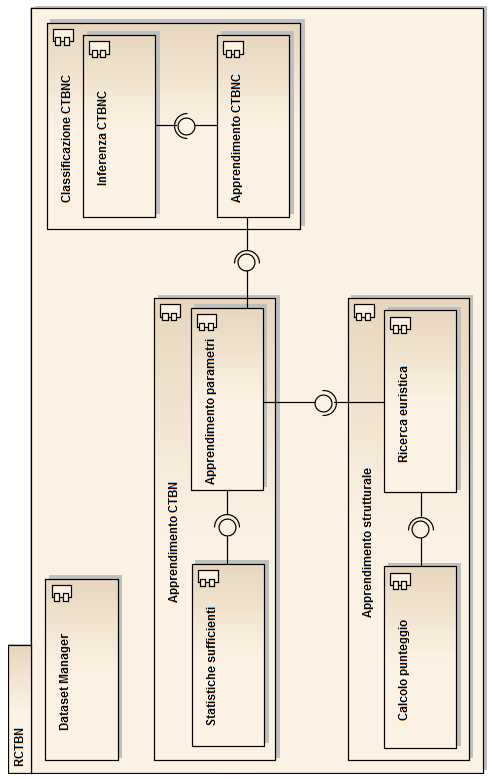
\includegraphics[width=1\columnwidth]{rctbn-arch.png}
	\caption[Diagramma dei componenti di \rctbn{}]{Diagramma dei componenti di \rctbn{}.}
	\label{fig:rctbncomponents}
\end{figure}

%\section{R}
%\omissis{}

%\section{Analisi}
%\omissis{}

%scopo
%vincoli: da chi deve essere usato? dove deve essere installato? attori? -> casi d'uso (con precondinzioni)
%requisiti: il sistema deve permettere ..
%tabella casi d'uso/requisiti?

%\section{Package CTBN}
%\omissis{}

%\subsection{Gestione dei dati}\label{subsec:rctbn-ds-management}
%\omissis{}

%\subsection{Apprendimento}\label{subsec:rctbn-learning}
%\omissis{}

%\subsection{Inferenza}\label{subsec:rctbn-inference}
%\omissis{}

%\subsection{Apprendimento strutturale}\label{subsec:rctbn-structurallearning}
%\omissis{}

%\subsection{Package xvalidation}\label{subsec:rctbn-xvalidation}
%\omissis{}

% introdurre R? Rcpp?
% introdurre paradigma funzionale?
% architettura/componenti
% signature + documentazione funzioni principali?
% parlare dei task che supportano la parallelizzazione
% struttura package R
% componente cross-validation: spiegare metriche di valutazione utilizzate? si! ma in capitolo 4!
